\documentclass[1p]{elsarticle_modified}
%\bibliographystyle{elsarticle-num}

%\usepackage[colorlinks]{hyperref}
%\usepackage{abbrmath_seonhwa} %\Abb, \Ascr, \Acal ,\Abf, \Afrak
\usepackage{amsfonts}
\usepackage{amssymb}
\usepackage{amsmath}
\usepackage{amsthm}
\usepackage{scalefnt}
\usepackage{amsbsy}
\usepackage{kotex}
\usepackage{caption}
\usepackage{subfig}
\usepackage{color}
\usepackage{graphicx}
\usepackage{xcolor} %% white, black, red, green, blue, cyan, magenta, yellow
\usepackage{float}
\usepackage{setspace}
\usepackage{hyperref}

\usepackage{tikz}
\usetikzlibrary{arrows}

\usepackage{multirow}
\usepackage{array} % fixed length table
\usepackage{hhline}

%%%%%%%%%%%%%%%%%%%%%
\makeatletter
\renewcommand*\env@matrix[1][\arraystretch]{%
	\edef\arraystretch{#1}%
	\hskip -\arraycolsep
	\let\@ifnextchar\new@ifnextchar
	\array{*\c@MaxMatrixCols c}}
\makeatother %https://tex.stackexchange.com/questions/14071/how-can-i-increase-the-line-spacing-in-a-matrix
%%%%%%%%%%%%%%%

\usepackage[normalem]{ulem}

\newcommand{\msout}[1]{\ifmmode\text{\sout{\ensuremath{#1}}}\else\sout{#1}\fi}
%SOURCE: \msout is \stkout macro in https://tex.stackexchange.com/questions/20609/strikeout-in-math-mode

\newcommand{\cancel}[1]{
	\ifmmode
	{\color{red}\msout{#1}}
	\else
	{\color{red}\sout{#1}}
	\fi
}

\newcommand{\add}[1]{
	{\color{blue}\uwave{#1}}
}

\newcommand{\replace}[2]{
	\ifmmode
	{\color{red}\msout{#1}}{\color{blue}\uwave{#2}}
	\else
	{\color{red}\sout{#1}}{\color{blue}\uwave{#2}}
	\fi
}

\newcommand{\Sol}{\mathcal{S}} %segment
\newcommand{\D}{D} %diagram
\newcommand{\A}{\mathcal{A}} %arc


%%%%%%%%%%%%%%%%%%%%%%%%%%%%%5 test

\def\sl{\operatorname{\textup{SL}}(2,\Cbb)}
\def\psl{\operatorname{\textup{PSL}}(2,\Cbb)}
\def\quan{\mkern 1mu \triangleright \mkern 1mu}

\theoremstyle{definition}
\newtheorem{thm}{Theorem}[section]
\newtheorem{prop}[thm]{Proposition}
\newtheorem{lem}[thm]{Lemma}
\newtheorem{ques}[thm]{Question}
\newtheorem{cor}[thm]{Corollary}
\newtheorem{defn}[thm]{Definition}
\newtheorem{exam}[thm]{Example}
\newtheorem{rmk}[thm]{Remark}
\newtheorem{alg}[thm]{Algorithm}

\newcommand{\I}{\sqrt{-1}}
\begin{document}

%\begin{frontmatter}
%
%\title{Boundary parabolic representations of knots up to 8 crossings}
%
%%% Group authors per affiliation:
%\author{Yunhi Cho} 
%\address{Department of Mathematics, University of Seoul, Seoul, Korea}
%\ead{yhcho@uos.ac.kr}
%
%
%\author{Seonhwa Kim} %\fnref{s_kim}}
%\address{Center for Geometry and Physics, Institute for Basic Science, Pohang, 37673, Korea}
%\ead{ryeona17@ibs.re.kr}
%
%\author{Hyuk Kim}
%\address{Department of Mathematical Sciences, Seoul National University, Seoul 08826, Korea}
%\ead{hyukkim@snu.ac.kr}
%
%\author{Seokbeom Yoon}
%\address{Department of Mathematical Sciences, Seoul National University, Seoul, 08826,  Korea}
%\ead{sbyoon15@snu.ac.kr}
%
%\begin{abstract}
%We find all boundary parabolic representation of knots up to 8 crossings.
%
%\end{abstract}
%\begin{keyword}
%    \MSC[2010] 57M25 
%\end{keyword}
%
%\end{frontmatter}

%\linenumbers
%\tableofcontents
%
\newcommand\colored[1]{\textcolor{white}{\rule[-0.35ex]{0.8em}{1.4ex}}\kern-0.8em\color{red} #1}%
%\newcommand\colored[1]{\textcolor{white}{ #1}\kern-2.17ex	\textcolor{white}{ #1}\kern-1.81ex	\textcolor{white}{ #1}\kern-2.15ex\color{red}#1	}

{\Large $\underline{12n_{0321}~(K12n_{0321})}$}

\setlength{\tabcolsep}{10pt}
\renewcommand{\arraystretch}{1.6}
\vspace{1cm}\begin{tabular}{m{100pt}>{\centering\arraybackslash}m{274pt}}
\multirow{5}{120pt}{
	\centering
	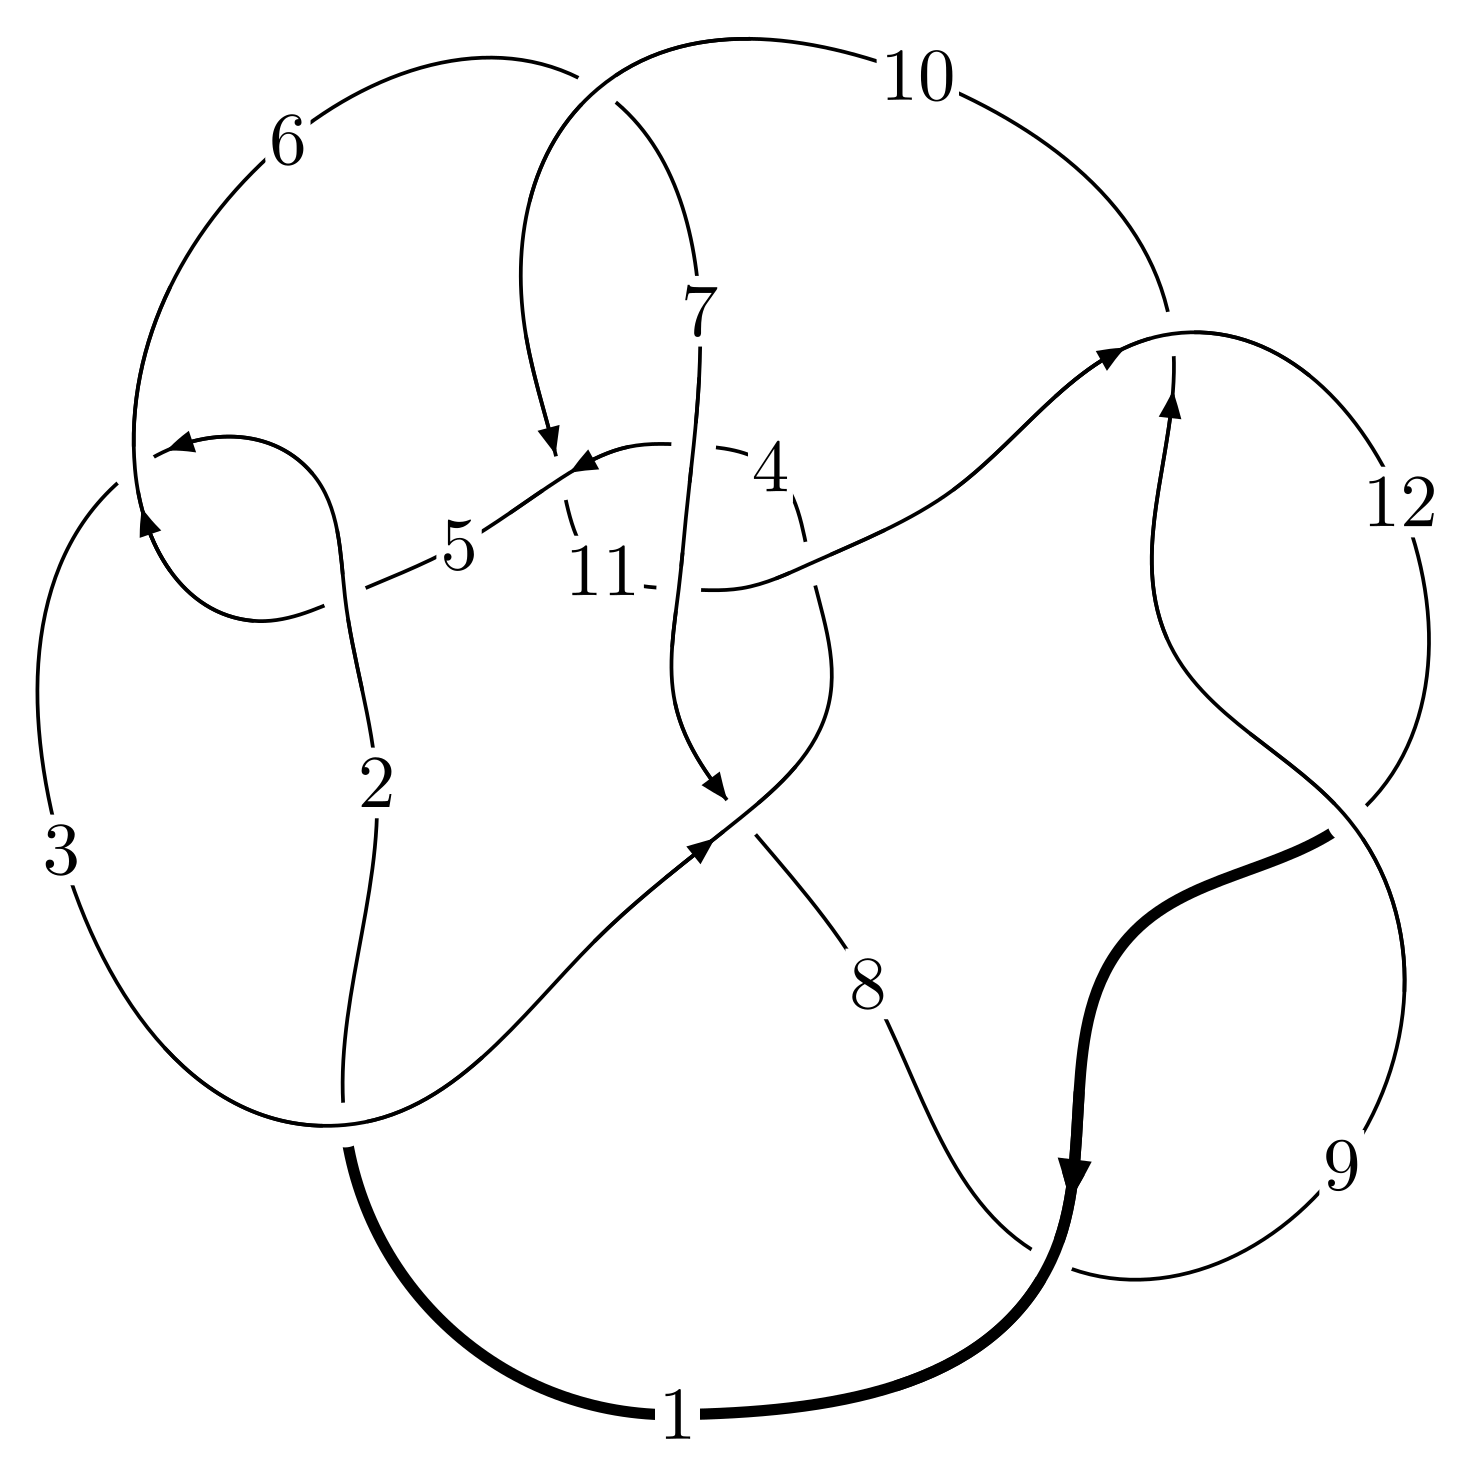
\includegraphics[width=112pt]{../../../GIT/diagram.site/Diagrams/png/2410_12n_0321.png}\\
\ \ \ A knot diagram\footnotemark}&
\allowdisplaybreaks
\textbf{Linearized knot diagam} \\
\cline{2-2}
 &
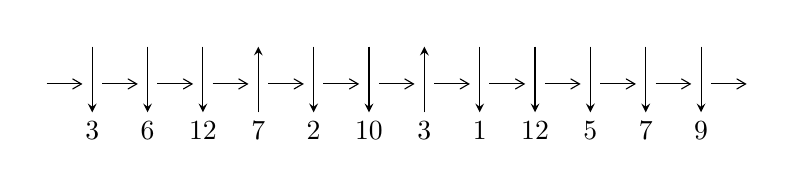
\begin{tikzpicture}[x=20pt, y=17pt]
	% nodes
	\node (C0) at (0, 0) {};
	\node (C1) at (1, 0) {};
	\node (C1U) at (1, +1) {};
	\node (C1D) at (1, -1) {3};

	\node (C2) at (2, 0) {};
	\node (C2U) at (2, +1) {};
	\node (C2D) at (2, -1) {6};

	\node (C3) at (3, 0) {};
	\node (C3U) at (3, +1) {};
	\node (C3D) at (3, -1) {12};

	\node (C4) at (4, 0) {};
	\node (C4U) at (4, +1) {};
	\node (C4D) at (4, -1) {7};

	\node (C5) at (5, 0) {};
	\node (C5U) at (5, +1) {};
	\node (C5D) at (5, -1) {2};

	\node (C6) at (6, 0) {};
	\node (C6U) at (6, +1) {};
	\node (C6D) at (6, -1) {10};

	\node (C7) at (7, 0) {};
	\node (C7U) at (7, +1) {};
	\node (C7D) at (7, -1) {3};

	\node (C8) at (8, 0) {};
	\node (C8U) at (8, +1) {};
	\node (C8D) at (8, -1) {1};

	\node (C9) at (9, 0) {};
	\node (C9U) at (9, +1) {};
	\node (C9D) at (9, -1) {12};

	\node (C10) at (10, 0) {};
	\node (C10U) at (10, +1) {};
	\node (C10D) at (10, -1) {5};

	\node (C11) at (11, 0) {};
	\node (C11U) at (11, +1) {};
	\node (C11D) at (11, -1) {7};

	\node (C12) at (12, 0) {};
	\node (C12U) at (12, +1) {};
	\node (C12D) at (12, -1) {9};
	\node (C13) at (13, 0) {};

	% arrows
	\draw[->,>={angle 60}]
	(C0) edge (C1) (C1) edge (C2) (C2) edge (C3) (C3) edge (C4) (C4) edge (C5) (C5) edge (C6) (C6) edge (C7) (C7) edge (C8) (C8) edge (C9) (C9) edge (C10) (C10) edge (C11) (C11) edge (C12) (C12) edge (C13) ;	\draw[->,>=stealth]
	(C1U) edge (C1D) (C2U) edge (C2D) (C3U) edge (C3D) (C4D) edge (C4U) (C5U) edge (C5D) (C6U) edge (C6D) (C7D) edge (C7U) (C8U) edge (C8D) (C9U) edge (C9D) (C10U) edge (C10D) (C11U) edge (C11D) (C12U) edge (C12D) ;
	\end{tikzpicture} \\
\hhline{~~} \\& 
\textbf{Solving Sequence} \\ \cline{2-2} 
 &
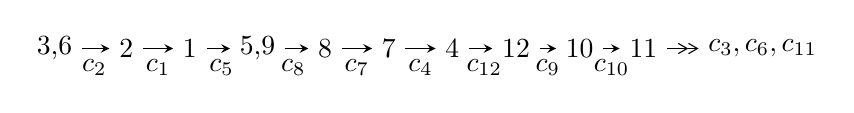
\begin{tikzpicture}[x=23pt, y=7pt]
	% node
	\node (A0) at (-1/8, 0) {3,6};
	\node (A1) at (1, 0) {2};
	\node (A2) at (2, 0) {1};
	\node (A3) at (49/16, 0) {5,9};
	\node (A4) at (33/8, 0) {8};
	\node (A5) at (41/8, 0) {7};
	\node (A6) at (49/8, 0) {4};
	\node (A7) at (57/8, 0) {12};
	\node (A8) at (65/8, 0) {10};
	\node (A9) at (73/8, 0) {11};
	\node (C1) at (1/2, -1) {$c_{2}$};
	\node (C2) at (3/2, -1) {$c_{1}$};
	\node (C3) at (5/2, -1) {$c_{5}$};
	\node (C4) at (29/8, -1) {$c_{8}$};
	\node (C5) at (37/8, -1) {$c_{7}$};
	\node (C6) at (45/8, -1) {$c_{4}$};
	\node (C7) at (53/8, -1) {$c_{12}$};
	\node (C8) at (61/8, -1) {$c_{9}$};
	\node (C9) at (69/8, -1) {$c_{10}$};
	\node (A10) at (11, 0) {$c_{3},c_{6},c_{11}$};

	% edge
	\draw[->,>=stealth]	
	(A0) edge (A1) (A1) edge (A2) (A2) edge (A3) (A3) edge (A4) (A4) edge (A5) (A5) edge (A6) (A6) edge (A7) (A7) edge (A8) (A8) edge (A9) ;
	\draw[->>,>={angle 60}]	
	(A9) edge (A10);
\end{tikzpicture} \\ 

\end{tabular} \\

\footnotetext{
The image of knot diagram is generated by the software ``\textbf{Draw programme}" developed by Andrew Bartholomew(\url{http://www.layer8.co.uk/maths/draw/index.htm\#Running-draw}), where we modified some parts for our purpose(\url{https://github.com/CATsTAILs/LinksPainter}).
}\phantom \\ \newline 
\centering \textbf{Ideals for irreducible components\footnotemark of $X_{\text{par}}$} 
 
\begin{align*}
I^u_{1}&=\langle 
-28 u^8+32 u^7-37 u^6-26 u^5-112 u^4-40 u^3-37 u^2+59 b+86 u-72,\\
\phantom{I^u_{1}}&\phantom{= \langle  }-7 u^8+8 u^7-24 u^6+23 u^5-28 u^4-69 u^3-24 u^2+59 a+110 u-18,\\
\phantom{I^u_{1}}&\phantom{= \langle  }u^9-2 u^8+2 u^7+u^6+2 u^5-2 u^4+u^3-3 u^2+4 u-1\rangle \\
I^u_{2}&=\langle 
- u^2+b- u+2,\;a+1,\;u^4+u^3- u^2- u+1\rangle \\
I^u_{3}&=\langle 
-2 u^7-3 u^6-2 u^5+4 u^4+7 u^3+5 u^2+b-5 u-5,\;-2 u^7-2 u^6- u^5+5 u^4+5 u^3+3 u^2+a-6 u-2,\\
\phantom{I^u_{3}}&\phantom{= \langle  }u^8+2 u^7+2 u^6- u^5-4 u^4-4 u^3+u^2+3 u+1\rangle \\
I^u_{4}&=\langle 
-3 u^5+u^3-11 u^2+19 b+7 u-18,\;-9 u^5+19 u^4-35 u^3+43 u^2+19 a-74 u+22,\\
\phantom{I^u_{4}}&\phantom{= \langle  }u^6-3 u^5+6 u^4-8 u^3+12 u^2-6 u+1\rangle \\
I^u_{5}&=\langle 
b,\;a+u+1,\;u^2+u+1\rangle \\
\\
\end{align*}
\raggedright * 5 irreducible components of $\dim_{\mathbb{C}}=0$, with total 29 representations.\\
\footnotetext{All coefficients of polynomials are rational numbers. But the coefficients are sometimes approximated in decimal forms when there is not enough margin.}
\newpage
\renewcommand{\arraystretch}{1}
\centering \section*{I. $I^u_{1}= \langle -28 u^8+32 u^7+\cdots+59 b-72,\;-7 u^8+8 u^7+\cdots+59 a-18,\;u^9-2 u^8+\cdots+4 u-1 \rangle$}
\flushleft \textbf{(i) Arc colorings}\\
\begin{tabular}{m{7pt} m{180pt} m{7pt} m{180pt} }
\flushright $a_{3}=$&$\begin{pmatrix}1\\0\end{pmatrix}$ \\
\flushright $a_{6}=$&$\begin{pmatrix}0\\u\end{pmatrix}$ \\
\flushright $a_{2}=$&$\begin{pmatrix}1\\- u^2\end{pmatrix}$ \\
\flushright $a_{1}=$&$\begin{pmatrix}- u^2+1\\- u^2\end{pmatrix}$ \\
\flushright $a_{5}=$&$\begin{pmatrix}u\\- u^3+u\end{pmatrix}$ \\
\flushright $a_{9}=$&$\begin{pmatrix}0.118644 u^{8}-0.135593 u^{7}+\cdots-1.86441 u+0.305085\\0.474576 u^{8}-0.542373 u^{7}+\cdots-1.45763 u+1.22034\end{pmatrix}$ \\
\flushright $a_{8}=$&$\begin{pmatrix}0.355932 u^{8}-0.406780 u^{7}+\cdots-1.59322 u+0.915254\\0.355932 u^{8}-0.406780 u^{7}+\cdots-0.593220 u+0.915254\end{pmatrix}$ \\
\flushright $a_{7}=$&$\begin{pmatrix}- u\\0.355932 u^{8}-0.406780 u^{7}+\cdots-0.593220 u+0.915254\end{pmatrix}$ \\
\flushright $a_{4}=$&$\begin{pmatrix}-0.118644 u^{8}+0.135593 u^{7}+\cdots+1.86441 u-0.305085\\0.440678 u^{8}-0.932203 u^{7}+\cdots-1.06780 u+0.847458\end{pmatrix}$ \\
\flushright $a_{12}=$&$\begin{pmatrix}0.389831 u^{8}-1.01695 u^{7}+\cdots-0.983051 u+1.28814\\-0.355932 u^{8}+0.406780 u^{7}+\cdots+0.593220 u-0.915254\end{pmatrix}$ \\
\flushright $a_{10}=$&$\begin{pmatrix}-1\\0.915254 u^{8}-1.47458 u^{7}+\cdots-2.52542 u+2.06780\end{pmatrix}$ \\
\flushright $a_{11}=$&$\begin{pmatrix}-0.305085 u^{8}+0.491525 u^{7}+\cdots+0.508475 u-1.35593\\0.711864 u^{8}-0.813559 u^{7}+\cdots-2.18644 u+1.83051\end{pmatrix}$\\&\end{tabular}
\flushleft \textbf{(ii) Obstruction class $= -1$}\\~\\
\flushleft \textbf{(iii) Cusp Shapes $= -\frac{15}{59} u^8+\frac{93}{59} u^7-\frac{43}{59} u^6-\frac{94}{59} u^5+\frac{235}{59} u^4+\frac{282}{59} u^3+\frac{193}{59} u^2-\frac{93}{59} u-\frac{342}{59}$}\\~\\
\newpage\renewcommand{\arraystretch}{1}
\flushleft \textbf{(iv) u-Polynomials at the component}\newline \\
\begin{tabular}{m{50pt}|m{274pt}}
Crossings & \hspace{64pt}u-Polynomials at each crossing \\
\hline $$\begin{aligned}c_{1}\end{aligned}$$&$\begin{aligned}
&u^9+12 u^7- u^6+8 u^5-18 u^4+7 u^3+5 u^2+10 u+1
\end{aligned}$\\
\hline $$\begin{aligned}c_{2},c_{5},c_{6}\end{aligned}$$&$\begin{aligned}
&u^9+2 u^8+2 u^7- u^6+2 u^5+2 u^4+u^3+3 u^2+4 u+1
\end{aligned}$\\
\hline $$\begin{aligned}c_{3},c_{8},c_{9}\\c_{10},c_{12}\end{aligned}$$&$\begin{aligned}
&u^9+7 u^7+5 u^6+15 u^5+13 u^4+11 u^3+7 u^2+u+1
\end{aligned}$\\
\hline $$\begin{aligned}c_{4}\end{aligned}$$&$\begin{aligned}
&u^9+2 u^8-7 u^7-15 u^6+13 u^5+53 u^4+71 u^3+61 u^2+29 u+5
\end{aligned}$\\
\hline $$\begin{aligned}c_{7}\end{aligned}$$&$\begin{aligned}
&u^9-7 u^8+5 u^7+42 u^6+92 u^5+125 u^4+125 u^3+88 u^2+39 u+9
\end{aligned}$\\
\hline $$\begin{aligned}c_{11}\end{aligned}$$&$\begin{aligned}
&u^9+u^8+14 u^7+10 u^6+39 u^5-44 u^4-45 u^3+4 u^2+20 u+9
\end{aligned}$\\
\hline
\end{tabular}\\~\\
\newpage\renewcommand{\arraystretch}{1}
\flushleft \textbf{(v) Riley Polynomials at the component}\newline \\
\begin{tabular}{m{50pt}|m{274pt}}
Crossings & \hspace{64pt}Riley Polynomials at each crossing \\
\hline $$\begin{aligned}c_{1}\end{aligned}$$&$\begin{aligned}
&y^9+24 y^8+\cdots+90 y-1
\end{aligned}$\\
\hline $$\begin{aligned}c_{2},c_{5},c_{6}\end{aligned}$$&$\begin{aligned}
&y^9+12 y^7+y^6+8 y^5+18 y^4+7 y^3-5 y^2+10 y-1
\end{aligned}$\\
\hline $$\begin{aligned}c_{3},c_{8},c_{9}\\c_{10},c_{12}\end{aligned}$$&$\begin{aligned}
&y^9+14 y^8+79 y^7+207 y^6+251 y^5+105 y^4-41 y^3-53 y^2-13 y-1
\end{aligned}$\\
\hline $$\begin{aligned}c_{4}\end{aligned}$$&$\begin{aligned}
&y^9-18 y^8+\cdots+231 y-25
\end{aligned}$\\
\hline $$\begin{aligned}c_{7}\end{aligned}$$&$\begin{aligned}
&y^9-39 y^8+\cdots-63 y-81
\end{aligned}$\\
\hline $$\begin{aligned}c_{11}\end{aligned}$$&$\begin{aligned}
&y^9+27 y^8+\cdots+328 y-81
\end{aligned}$\\
\hline
\end{tabular}\\~\\
\newpage\flushleft \textbf{(vi) Complex Volumes and Cusp Shapes}
$$\begin{array}{c|c|c}  
\text{Solutions to }I^u_{1}& \I (\text{vol} + \sqrt{-1}CS) & \text{Cusp shape}\\
 \hline 
\begin{aligned}
u &= -0.236649 + 0.987655 I \\
a &= \phantom{-}1.59024 - 3.04254 I \\
b &= \phantom{-}1.32330 - 0.67194 I\end{aligned}
 & \phantom{-}9.89350 + 2.31667 I & \phantom{-}0.86831 - 3.48815 I \\ \hline\begin{aligned}
u &= -0.236649 - 0.987655 I \\
a &= \phantom{-}1.59024 + 3.04254 I \\
b &= \phantom{-}1.32330 + 0.67194 I\end{aligned}
 & \phantom{-}9.89350 - 2.31667 I & \phantom{-}0.86831 + 3.48815 I \\ \hline\begin{aligned}
u &= -0.948444 + 0.610151 I \\
a &= \phantom{-}0.291757 + 0.057514 I \\
b &= -0.400025 - 0.194724 I\end{aligned}
 & \phantom{-}1.50288 + 4.69117 I & -4.69492 - 7.49384 I \\ \hline\begin{aligned}
u &= -0.948444 - 0.610151 I \\
a &= \phantom{-}0.291757 - 0.057514 I \\
b &= -0.400025 + 0.194724 I\end{aligned}
 & \phantom{-}1.50288 - 4.69117 I & -4.69492 + 7.49384 I \\ \hline\begin{aligned}
u &= \phantom{-}0.731097 + 0.406841 I \\
a &= -0.967602 + 0.291558 I \\
b &= -0.297854 + 1.104540 I\end{aligned}
 & -1.11949 - 1.41007 I & -6.06702 + 5.32264 I \\ \hline\begin{aligned}
u &= \phantom{-}0.731097 - 0.406841 I \\
a &= -0.967602 - 0.291558 I \\
b &= -0.297854 - 1.104540 I\end{aligned}
 & -1.11949 + 1.41007 I & -6.06702 - 5.32264 I \\ \hline\begin{aligned}
u &= \phantom{-}0.323158\phantom{ +0.000000I} \\
a &= -0.211236\phantom{ +0.000000I} \\
b &= \phantom{-}0.860492\phantom{ +0.000000I}\end{aligned}
 & -1.09696\phantom{ +0.000000I} & -5.76550\phantom{ +0.000000I} \\ \hline\begin{aligned}
u &= \phantom{-}1.29242 + 1.30359 I \\
a &= \phantom{-}1.69122 + 1.25994 I \\
b &= \phantom{-}2.44434 + 0.36799 I\end{aligned}
 & -13.8407 - 9.8067 I & -4.22361 + 3.66185 I \\ \hline\begin{aligned}
u &= \phantom{-}1.29242 - 1.30359 I \\
a &= \phantom{-}1.69122 - 1.25994 I \\
b &= \phantom{-}2.44434 - 0.36799 I\end{aligned}
 & -13.8407 + 9.8067 I & -4.22361 - 3.66185 I\\
 \hline 
 \end{array}$$\newpage\newpage\renewcommand{\arraystretch}{1}
\centering \section*{II. $I^u_{2}= \langle - u^2+b- u+2,\;a+1,\;u^4+u^3- u^2- u+1 \rangle$}
\flushleft \textbf{(i) Arc colorings}\\
\begin{tabular}{m{7pt} m{180pt} m{7pt} m{180pt} }
\flushright $a_{3}=$&$\begin{pmatrix}1\\0\end{pmatrix}$ \\
\flushright $a_{6}=$&$\begin{pmatrix}0\\u\end{pmatrix}$ \\
\flushright $a_{2}=$&$\begin{pmatrix}1\\- u^2\end{pmatrix}$ \\
\flushright $a_{1}=$&$\begin{pmatrix}- u^2+1\\- u^2\end{pmatrix}$ \\
\flushright $a_{5}=$&$\begin{pmatrix}u\\- u^3+u\end{pmatrix}$ \\
\flushright $a_{9}=$&$\begin{pmatrix}-1\\u^2+u-2\end{pmatrix}$ \\
\flushright $a_{8}=$&$\begin{pmatrix}u^3+u^2- u-1\\u^3+u^2-1\end{pmatrix}$ \\
\flushright $a_{7}=$&$\begin{pmatrix}- u\\u^3+u^2-1\end{pmatrix}$ \\
\flushright $a_{4}=$&$\begin{pmatrix}1\\- u^3- u^2+u\end{pmatrix}$ \\
\flushright $a_{12}=$&$\begin{pmatrix}0\\u^2-1\end{pmatrix}$ \\
\flushright $a_{10}=$&$\begin{pmatrix}-1\\u^3+2 u^2-2\end{pmatrix}$ \\
\flushright $a_{11}=$&$\begin{pmatrix}- u^3+u-1\\u^3+2 u^2- u-1\end{pmatrix}$\\&\end{tabular}
\flushleft \textbf{(ii) Obstruction class $= 1$}\\~\\
\flushleft \textbf{(iii) Cusp Shapes $= 2 u^3+5 u^2-3 u-13$}\\~\\
\newpage\renewcommand{\arraystretch}{1}
\flushleft \textbf{(iv) u-Polynomials at the component}\newline \\
\begin{tabular}{m{50pt}|m{274pt}}
Crossings & \hspace{64pt}u-Polynomials at each crossing \\
\hline $$\begin{aligned}c_{1}\end{aligned}$$&$\begin{aligned}
&u^4-3 u^3+5 u^2-3 u+1
\end{aligned}$\\
\hline $$\begin{aligned}c_{2},c_{6}\end{aligned}$$&$\begin{aligned}
&u^4+u^3- u^2- u+1
\end{aligned}$\\
\hline $$\begin{aligned}c_{3},c_{12}\end{aligned}$$&$\begin{aligned}
&u^4+u^3+2 u^2+2 u+1
\end{aligned}$\\
\hline $$\begin{aligned}c_{4}\end{aligned}$$&$\begin{aligned}
&u^4-3 u^3+2 u^2+1
\end{aligned}$\\
\hline $$\begin{aligned}c_{5}\end{aligned}$$&$\begin{aligned}
&u^4- u^3- u^2+u+1
\end{aligned}$\\
\hline $$\begin{aligned}c_{7}\end{aligned}$$&$\begin{aligned}
&(u^2- u+1)^2
\end{aligned}$\\
\hline $$\begin{aligned}c_{8},c_{9},c_{10}\end{aligned}$$&$\begin{aligned}
&u^4- u^3+2 u^2-2 u+1
\end{aligned}$\\
\hline $$\begin{aligned}c_{11}\end{aligned}$$&$\begin{aligned}
&u^4+2 u^2+3 u+1
\end{aligned}$\\
\hline
\end{tabular}\\~\\
\newpage\renewcommand{\arraystretch}{1}
\flushleft \textbf{(v) Riley Polynomials at the component}\newline \\
\begin{tabular}{m{50pt}|m{274pt}}
Crossings & \hspace{64pt}Riley Polynomials at each crossing \\
\hline $$\begin{aligned}c_{1}\end{aligned}$$&$\begin{aligned}
&y^4+y^3+9 y^2+y+1
\end{aligned}$\\
\hline $$\begin{aligned}c_{2},c_{5},c_{6}\end{aligned}$$&$\begin{aligned}
&y^4-3 y^3+5 y^2-3 y+1
\end{aligned}$\\
\hline $$\begin{aligned}c_{3},c_{8},c_{9}\\c_{10},c_{12}\end{aligned}$$&$\begin{aligned}
&y^4+3 y^3+2 y^2+1
\end{aligned}$\\
\hline $$\begin{aligned}c_{4}\end{aligned}$$&$\begin{aligned}
&y^4-5 y^3+6 y^2+4 y+1
\end{aligned}$\\
\hline $$\begin{aligned}c_{7}\end{aligned}$$&$\begin{aligned}
&(y^2+y+1)^2
\end{aligned}$\\
\hline $$\begin{aligned}c_{11}\end{aligned}$$&$\begin{aligned}
&y^4+4 y^3+6 y^2-5 y+1
\end{aligned}$\\
\hline
\end{tabular}\\~\\
\newpage\flushleft \textbf{(vi) Complex Volumes and Cusp Shapes}
$$\begin{array}{c|c|c}  
\text{Solutions to }I^u_{2}& \I (\text{vol} + \sqrt{-1}CS) & \text{Cusp shape}\\
 \hline 
\begin{aligned}
u &= \phantom{-}0.692440 + 0.318148 I \\
a &= -1.00000\phantom{ +0.000000I} \\
b &= -0.929304 + 0.758745 I\end{aligned}
 & -1.74699 - 0.56550 I & -12.94255 + 2.09940 I \\ \hline\begin{aligned}
u &= \phantom{-}0.692440 - 0.318148 I \\
a &= -1.00000\phantom{ +0.000000I} \\
b &= -0.929304 - 0.758745 I\end{aligned}
 & -1.74699 + 0.56550 I & -12.94255 - 2.09940 I \\ \hline\begin{aligned}
u &= -1.192440 + 0.547877 I \\
a &= -1.00000\phantom{ +0.000000I} \\
b &= -2.07070 - 0.75874 I\end{aligned}
 & \phantom{-}5.03685 + 4.62527 I & -5.05745 - 3.83145 I \\ \hline\begin{aligned}
u &= -1.192440 - 0.547877 I \\
a &= -1.00000\phantom{ +0.000000I} \\
b &= -2.07070 + 0.75874 I\end{aligned}
 & \phantom{-}5.03685 - 4.62527 I & -5.05745 + 3.83145 I\\
 \hline 
 \end{array}$$\newpage\newpage\renewcommand{\arraystretch}{1}
\centering \section*{III. $I^u_{3}= \langle -2 u^7-3 u^6+\cdots+b-5,\;-2 u^7-2 u^6+\cdots+a-2,\;u^8+2 u^7+2 u^6- u^5-4 u^4-4 u^3+u^2+3 u+1 \rangle$}
\flushleft \textbf{(i) Arc colorings}\\
\begin{tabular}{m{7pt} m{180pt} m{7pt} m{180pt} }
\flushright $a_{3}=$&$\begin{pmatrix}1\\0\end{pmatrix}$ \\
\flushright $a_{6}=$&$\begin{pmatrix}0\\u\end{pmatrix}$ \\
\flushright $a_{2}=$&$\begin{pmatrix}1\\- u^2\end{pmatrix}$ \\
\flushright $a_{1}=$&$\begin{pmatrix}- u^2+1\\- u^2\end{pmatrix}$ \\
\flushright $a_{5}=$&$\begin{pmatrix}u\\- u^3+u\end{pmatrix}$ \\
\flushright $a_{9}=$&$\begin{pmatrix}2 u^7+2 u^6+u^5-5 u^4-5 u^3-3 u^2+6 u+2\\2 u^7+3 u^6+2 u^5-4 u^4-7 u^3-5 u^2+5 u+5\end{pmatrix}$ \\
\flushright $a_{8}=$&$\begin{pmatrix}4 u^7+5 u^6+4 u^5-8 u^4-12 u^3-9 u^2+11 u+6\\u^7+2 u^6+2 u^5- u^4-4 u^3-4 u^2+2 u+3\end{pmatrix}$ \\
\flushright $a_{7}=$&$\begin{pmatrix}3 u^7+3 u^6+2 u^5-7 u^4-8 u^3-5 u^2+9 u+3\\u^7+2 u^6+2 u^5- u^4-4 u^3-4 u^2+2 u+3\end{pmatrix}$ \\
\flushright $a_{4}=$&$\begin{pmatrix}-10 u^7-13 u^6-11 u^5+17 u^4+27 u^3+20 u^2-23 u-12\\- u^7-2 u^6-2 u^5+u^4+4 u^3+4 u^2- u-4\end{pmatrix}$ \\
\flushright $a_{12}=$&$\begin{pmatrix}6 u^7+9 u^6+7 u^5-11 u^4-20 u^3-14 u^2+15 u+13\\-5 u^7-7 u^6-6 u^5+8 u^4+15 u^3+11 u^2-11 u-8\end{pmatrix}$ \\
\flushright $a_{10}=$&$\begin{pmatrix}-7 u^7-10 u^6-8 u^5+12 u^4+22 u^3+16 u^2-16 u-12\\3 u^7+4 u^6+3 u^5-6 u^4-9 u^3-6 u^2+8 u+5\end{pmatrix}$ \\
\flushright $a_{11}=$&$\begin{pmatrix}-10 u^7-14 u^6-11 u^5+17 u^4+31 u^3+22 u^2-23 u-17\\u^7+2 u^6+u^5-3 u^4-4 u^3-2 u^2+4 u+2\end{pmatrix}$\\&\end{tabular}
\flushleft \textbf{(ii) Obstruction class $= 1$}\\~\\
\flushleft \textbf{(iii) Cusp Shapes $= 2 u^7+3 u^6+3 u^5-2 u^4-5 u^3-4 u^2+3 u-2$}\\~\\
\newpage\renewcommand{\arraystretch}{1}
\flushleft \textbf{(iv) u-Polynomials at the component}\newline \\
\begin{tabular}{m{50pt}|m{274pt}}
Crossings & \hspace{64pt}u-Polynomials at each crossing \\
\hline $$\begin{aligned}c_{1}\end{aligned}$$&$\begin{aligned}
&u^8+u^5+2 u^4-14 u^3+17 u^2-7 u+1
\end{aligned}$\\
\hline $$\begin{aligned}c_{2},c_{6}\end{aligned}$$&$\begin{aligned}
&u^8+2 u^7+2 u^6- u^5-4 u^4-4 u^3+u^2+3 u+1
\end{aligned}$\\
\hline $$\begin{aligned}c_{3},c_{12}\end{aligned}$$&$\begin{aligned}
&u^8- u^7+6 u^6-5 u^5+12 u^4-8 u^3+9 u^2-4 u+1
\end{aligned}$\\
\hline $$\begin{aligned}c_{4}\end{aligned}$$&$\begin{aligned}
&(u^4+3 u^3+u^2-2 u+1)^2
\end{aligned}$\\
\hline $$\begin{aligned}c_{5}\end{aligned}$$&$\begin{aligned}
&u^8-2 u^7+2 u^6+u^5-4 u^4+4 u^3+u^2-3 u+1
\end{aligned}$\\
\hline $$\begin{aligned}c_{7}\end{aligned}$$&$\begin{aligned}
&u^8+u^7+5 u^6+8 u^5+7 u^4+11 u^3+10 u^2+1
\end{aligned}$\\
\hline $$\begin{aligned}c_{8},c_{9},c_{10}\end{aligned}$$&$\begin{aligned}
&u^8+u^7+6 u^6+5 u^5+12 u^4+8 u^3+9 u^2+4 u+1
\end{aligned}$\\
\hline $$\begin{aligned}c_{11}\end{aligned}$$&$\begin{aligned}
&u^8-2 u^7+5 u^6+3 u^5+4 u^4+27 u^3-3 u^2-16 u+52
\end{aligned}$\\
\hline
\end{tabular}\\~\\
\newpage\renewcommand{\arraystretch}{1}
\flushleft \textbf{(v) Riley Polynomials at the component}\newline \\
\begin{tabular}{m{50pt}|m{274pt}}
Crossings & \hspace{64pt}Riley Polynomials at each crossing \\
\hline $$\begin{aligned}c_{1}\end{aligned}$$&$\begin{aligned}
&y^8+4 y^6+33 y^5+34 y^4-114 y^3+97 y^2-15 y+1
\end{aligned}$\\
\hline $$\begin{aligned}c_{2},c_{5},c_{6}\end{aligned}$$&$\begin{aligned}
&y^8+y^5+2 y^4-14 y^3+17 y^2-7 y+1
\end{aligned}$\\
\hline $$\begin{aligned}c_{3},c_{8},c_{9}\\c_{10},c_{12}\end{aligned}$$&$\begin{aligned}
&y^8+11 y^7+50 y^6+121 y^5+166 y^4+124 y^3+41 y^2+2 y+1
\end{aligned}$\\
\hline $$\begin{aligned}c_{4}\end{aligned}$$&$\begin{aligned}
&(y^4-7 y^3+15 y^2-2 y+1)^2
\end{aligned}$\\
\hline $$\begin{aligned}c_{7}\end{aligned}$$&$\begin{aligned}
&y^8+9 y^7+23 y^6+4 y^5-25 y^4+29 y^3+114 y^2+20 y+1
\end{aligned}$\\
\hline $$\begin{aligned}c_{11}\end{aligned}$$&$\begin{aligned}
&y^8+6 y^7+45 y^6+133 y^5-136 y^4-137 y^3+1289 y^2-568 y+2704
\end{aligned}$\\
\hline
\end{tabular}\\~\\
\newpage\flushleft \textbf{(vi) Complex Volumes and Cusp Shapes}
$$\begin{array}{c|c|c}  
\text{Solutions to }I^u_{3}& \I (\text{vol} + \sqrt{-1}CS) & \text{Cusp shape}\\
 \hline 
\begin{aligned}
u &= \phantom{-}0.963269 + 0.149069 I \\
a &= -0.307661 - 1.178810 I \\
b &= \phantom{-}0.148192 - 0.911292 I\end{aligned}
 & \phantom{-}1.43393 - 3.16396 I & -4.10488 + 1.55249 I \\ \hline\begin{aligned}
u &= \phantom{-}0.963269 - 0.149069 I \\
a &= -0.307661 + 1.178810 I \\
b &= \phantom{-}0.148192 + 0.911292 I\end{aligned}
 & \phantom{-}1.43393 + 3.16396 I & -4.10488 - 1.55249 I \\ \hline\begin{aligned}
u &= -1.006590 + 0.790269 I \\
a &= \phantom{-}0.550701 + 0.903791 I \\
b &= \phantom{-}0.148192 + 0.911292 I\end{aligned}
 & \phantom{-}1.43393 + 3.16396 I & -4.10488 - 1.55249 I \\ \hline\begin{aligned}
u &= -1.006590 - 0.790269 I \\
a &= \phantom{-}0.550701 - 0.903791 I \\
b &= \phantom{-}0.148192 - 0.911292 I\end{aligned}
 & \phantom{-}1.43393 - 3.16396 I & -4.10488 + 1.55249 I \\ \hline\begin{aligned}
u &= -0.384833 + 1.326500 I \\
a &= \phantom{-}1.24719 - 2.12175 I \\
b &= \phantom{-}1.35181 - 0.72034 I\end{aligned}
 & \phantom{-}8.43568 + 1.41510 I & -4.39512 - 0.50684 I \\ \hline\begin{aligned}
u &= -0.384833 - 1.326500 I \\
a &= \phantom{-}1.24719 + 2.12175 I \\
b &= \phantom{-}1.35181 + 0.72034 I\end{aligned}
 & \phantom{-}8.43568 - 1.41510 I & -4.39512 + 0.50684 I \\ \hline\begin{aligned}
u &= -0.571852 + 0.099314 I \\
a &= -1.99023 + 0.84034 I \\
b &= \phantom{-}1.35181 + 0.72034 I\end{aligned}
 & \phantom{-}8.43568 - 1.41510 I & -4.39512 + 0.50684 I \\ \hline\begin{aligned}
u &= -0.571852 - 0.099314 I \\
a &= -1.99023 - 0.84034 I \\
b &= \phantom{-}1.35181 - 0.72034 I\end{aligned}
 & \phantom{-}8.43568 + 1.41510 I & -4.39512 - 0.50684 I\\
 \hline 
 \end{array}$$\newpage\newpage\renewcommand{\arraystretch}{1}
\centering \section*{IV. $I^u_{4}= \langle -3 u^5+u^3-11 u^2+19 b+7 u-18,\;-9 u^5+19 u^4+\cdots+19 a+22,\;u^6-3 u^5+6 u^4-8 u^3+12 u^2-6 u+1 \rangle$}
\flushleft \textbf{(i) Arc colorings}\\
\begin{tabular}{m{7pt} m{180pt} m{7pt} m{180pt} }
\flushright $a_{3}=$&$\begin{pmatrix}1\\0\end{pmatrix}$ \\
\flushright $a_{6}=$&$\begin{pmatrix}0\\u\end{pmatrix}$ \\
\flushright $a_{2}=$&$\begin{pmatrix}1\\- u^2\end{pmatrix}$ \\
\flushright $a_{1}=$&$\begin{pmatrix}- u^2+1\\- u^2\end{pmatrix}$ \\
\flushright $a_{5}=$&$\begin{pmatrix}u\\- u^3+u\end{pmatrix}$ \\
\flushright $a_{9}=$&$\begin{pmatrix}\frac{9}{19} u^5- u^4+\cdots+\frac{74}{19} u-\frac{22}{19}\\0.157895 u^{5}-0.0526316 u^{3}+\cdots-0.368421 u+0.947368\end{pmatrix}$ \\
\flushright $a_{8}=$&$\begin{pmatrix}\frac{9}{19} u^5-2 u^4+\cdots+\frac{55}{19} u-\frac{3}{19}\\\frac{3}{19} u^5- u^4+\cdots-\frac{7}{19} u+\frac{18}{19}\end{pmatrix}$ \\
\flushright $a_{7}=$&$\begin{pmatrix}\frac{6}{19} u^5- u^4+\cdots+\frac{62}{19} u-\frac{21}{19}\\\frac{3}{19} u^5- u^4+\cdots-\frac{7}{19} u+\frac{18}{19}\end{pmatrix}$ \\
\flushright $a_{4}=$&$\begin{pmatrix}\frac{8}{19} u^5- u^4+\cdots+\frac{51}{19} u-\frac{9}{19}\\\frac{11}{19} u^5- u^4+\cdots+\frac{6}{19} u+\frac{9}{19}\end{pmatrix}$ \\
\flushright $a_{12}=$&$\begin{pmatrix}-\frac{6}{19} u^5+u^4+\cdots-\frac{81}{19} u+\frac{40}{19}\\-0.105263 u^{5}+0.368421 u^{3}+\cdots-0.421053 u-0.631579\end{pmatrix}$ \\
\flushright $a_{10}=$&$\begin{pmatrix}0.684211 u^{5}-2 u^{4}+\cdots+7.73684 u-2.89474\\-0.105263 u^{5}+0.368421 u^{3}+\cdots+0.578947 u+1.36842\end{pmatrix}$ \\
\flushright $a_{11}=$&$\begin{pmatrix}\frac{7}{19} u^5- u^4+\cdots+\frac{123}{19} u-\frac{53}{19}\\-1.57895 u^{5}+3 u^{4}+\cdots-1.31579 u+1.52632\end{pmatrix}$\\&\end{tabular}
\flushleft \textbf{(ii) Obstruction class $= -1$}\\~\\
\flushleft \textbf{(iii) Cusp Shapes $= -\frac{2}{19} u^5+\frac{7}{19} u^3-\frac{20}{19} u^2+\frac{11}{19} u-\frac{107}{19}$}\\~\\
\newpage\renewcommand{\arraystretch}{1}
\flushleft \textbf{(iv) u-Polynomials at the component}\newline \\
\begin{tabular}{m{50pt}|m{274pt}}
Crossings & \hspace{64pt}u-Polynomials at each crossing \\
\hline $$\begin{aligned}c_{1}\end{aligned}$$&$\begin{aligned}
&u^6-3 u^5+12 u^4-46 u^3+60 u^2+12 u+1
\end{aligned}$\\
\hline $$\begin{aligned}c_{2},c_{5},c_{6}\end{aligned}$$&$\begin{aligned}
&u^6+3 u^5+6 u^4+8 u^3+12 u^2+6 u+1
\end{aligned}$\\
\hline $$\begin{aligned}c_{3},c_{8},c_{9}\\c_{10},c_{12}\end{aligned}$$&$\begin{aligned}
&u^6+9 u^4+8 u^3+27 u^2+45 u+19
\end{aligned}$\\
\hline $$\begin{aligned}c_{4}\end{aligned}$$&$\begin{aligned}
&(u^3-3 u-1)^2
\end{aligned}$\\
\hline $$\begin{aligned}c_{7}\end{aligned}$$&$\begin{aligned}
&u^6+9 u^5+48 u^4+349 u^3+1647 u^2+2058 u+757
\end{aligned}$\\
\hline $$\begin{aligned}c_{11}\end{aligned}$$&$\begin{aligned}
&u^6+9 u^4-9 u^3+54 u^2+81 u+27
\end{aligned}$\\
\hline
\end{tabular}\\~\\
\newpage\renewcommand{\arraystretch}{1}
\flushleft \textbf{(v) Riley Polynomials at the component}\newline \\
\begin{tabular}{m{50pt}|m{274pt}}
Crossings & \hspace{64pt}Riley Polynomials at each crossing \\
\hline $$\begin{aligned}c_{1}\end{aligned}$$&$\begin{aligned}
&y^6+15 y^5-12 y^4-602 y^3+4728 y^2-24 y+1
\end{aligned}$\\
\hline $$\begin{aligned}c_{2},c_{5},c_{6}\end{aligned}$$&$\begin{aligned}
&y^6+3 y^5+12 y^4+46 y^3+60 y^2-12 y+1
\end{aligned}$\\
\hline $$\begin{aligned}c_{3},c_{8},c_{9}\\c_{10},c_{12}\end{aligned}$$&$\begin{aligned}
&y^6+18 y^5+135 y^4+460 y^3+351 y^2-999 y+361
\end{aligned}$\\
\hline $$\begin{aligned}c_{4}\end{aligned}$$&$\begin{aligned}
&(y^3-6 y^2+9 y-1)^2
\end{aligned}$\\
\hline $$\begin{aligned}c_{7}\end{aligned}$$&$\begin{aligned}
&y^6+15 y^5-684 y^4+781 y^3+1348797 y^2-1741806 y+573049
\end{aligned}$\\
\hline $$\begin{aligned}c_{11}\end{aligned}$$&$\begin{aligned}
&y^6+18 y^5+189 y^4+945 y^3+4860 y^2-3645 y+729
\end{aligned}$\\
\hline
\end{tabular}\\~\\
\newpage\flushleft \textbf{(vi) Complex Volumes and Cusp Shapes}
$$\begin{array}{c|c|c}  
\text{Solutions to }I^u_{4}& \I (\text{vol} + \sqrt{-1}CS) & \text{Cusp shape}\\
 \hline 
\begin{aligned}
u &= -0.26604 + 1.50881 I \\
a &= -1.17365 + 0.98481 I \\
b &= -1.34730\phantom{ +0.000000I}\end{aligned}
 & \phantom{-}12.0628\phantom{ +0.000000I} & -2.12061 + 0. I\phantom{ +0.000000I} \\ \hline\begin{aligned}
u &= -0.26604 - 1.50881 I \\
a &= -1.17365 - 0.98481 I \\
b &= -1.34730\phantom{ +0.000000I}\end{aligned}
 & \phantom{-}12.0628\phantom{ +0.000000I} & -2.12061 + 0. I\phantom{ +0.000000I} \\ \hline\begin{aligned}
u &= \phantom{-}0.326352 + 0.118782 I \\
a &= -0.060307 + 0.342020 I \\
b &= \phantom{-}0.879385\phantom{ +0.000000I}\end{aligned}
 & -1.09662\phantom{ +0.000000I} & -5.53209 + 0. I\phantom{ +0.000000I} \\ \hline\begin{aligned}
u &= \phantom{-}0.326352 - 0.118782 I \\
a &= -0.060307 - 0.342020 I \\
b &= \phantom{-}0.879385\phantom{ +0.000000I}\end{aligned}
 & -1.09662\phantom{ +0.000000I} & -5.53209 + 0. I\phantom{ +0.000000I} \\ \hline\begin{aligned}
u &= \phantom{-}1.43969 + 1.20805 I \\
a &= -1.76604 - 0.64279 I \\
b &= -2.53209\phantom{ +0.000000I}\end{aligned}
 & -14.2561\phantom{ +0.000000I} & -4.34730 + 0. I\phantom{ +0.000000I} \\ \hline\begin{aligned}
u &= \phantom{-}1.43969 - 1.20805 I \\
a &= -1.76604 + 0.64279 I \\
b &= -2.53209\phantom{ +0.000000I}\end{aligned}
 & -14.2561\phantom{ +0.000000I} & -4.34730 + 0. I\phantom{ +0.000000I}\\
 \hline 
 \end{array}$$\newpage\newpage\renewcommand{\arraystretch}{1}
\centering \section*{V. $I^u_{5}= \langle b,\;a+u+1,\;u^2+u+1 \rangle$}
\flushleft \textbf{(i) Arc colorings}\\
\begin{tabular}{m{7pt} m{180pt} m{7pt} m{180pt} }
\flushright $a_{3}=$&$\begin{pmatrix}1\\0\end{pmatrix}$ \\
\flushright $a_{6}=$&$\begin{pmatrix}0\\u\end{pmatrix}$ \\
\flushright $a_{2}=$&$\begin{pmatrix}1\\u+1\end{pmatrix}$ \\
\flushright $a_{1}=$&$\begin{pmatrix}u+2\\u+1\end{pmatrix}$ \\
\flushright $a_{5}=$&$\begin{pmatrix}u\\u-1\end{pmatrix}$ \\
\flushright $a_{9}=$&$\begin{pmatrix}- u-1\\0\end{pmatrix}$ \\
\flushright $a_{8}=$&$\begin{pmatrix}-2\\-1\end{pmatrix}$ \\
\flushright $a_{7}=$&$\begin{pmatrix}-1\\-1\end{pmatrix}$ \\
\flushright $a_{4}=$&$\begin{pmatrix}u+1\\u\end{pmatrix}$ \\
\flushright $a_{12}=$&$\begin{pmatrix}u+1\\u+1\end{pmatrix}$ \\
\flushright $a_{10}=$&$\begin{pmatrix}- u\\1\end{pmatrix}$ \\
\flushright $a_{11}=$&$\begin{pmatrix}- u-1\\- u-1\end{pmatrix}$\\&\end{tabular}
\flushleft \textbf{(ii) Obstruction class $= -1$}\\~\\
\flushleft \textbf{(iii) Cusp Shapes $= -3$}\\~\\
\newpage\renewcommand{\arraystretch}{1}
\flushleft \textbf{(iv) u-Polynomials at the component}\newline \\
\begin{tabular}{m{50pt}|m{274pt}}
Crossings & \hspace{64pt}u-Polynomials at each crossing \\
\hline $$\begin{aligned}c_{1},c_{2},c_{3}\\c_{5},c_{6},c_{8}\\c_{9},c_{10},c_{12}\end{aligned}$$&$\begin{aligned}
&u^2- u+1
\end{aligned}$\\
\hline $$\begin{aligned}c_{4},c_{7}\end{aligned}$$&$\begin{aligned}
&(u-1)^2
\end{aligned}$\\
\hline $$\begin{aligned}c_{11}\end{aligned}$$&$\begin{aligned}
&u^2
\end{aligned}$\\
\hline
\end{tabular}\\~\\
\newpage\renewcommand{\arraystretch}{1}
\flushleft \textbf{(v) Riley Polynomials at the component}\newline \\
\begin{tabular}{m{50pt}|m{274pt}}
Crossings & \hspace{64pt}Riley Polynomials at each crossing \\
\hline $$\begin{aligned}c_{1},c_{2},c_{3}\\c_{5},c_{6},c_{8}\\c_{9},c_{10},c_{12}\end{aligned}$$&$\begin{aligned}
&y^2+y+1
\end{aligned}$\\
\hline $$\begin{aligned}c_{4},c_{7}\end{aligned}$$&$\begin{aligned}
&(y-1)^2
\end{aligned}$\\
\hline $$\begin{aligned}c_{11}\end{aligned}$$&$\begin{aligned}
&y^2
\end{aligned}$\\
\hline
\end{tabular}\\~\\
\newpage\flushleft \textbf{(vi) Complex Volumes and Cusp Shapes}
$$\begin{array}{c|c|c}  
\text{Solutions to }I^u_{5}& \I (\text{vol} + \sqrt{-1}CS) & \text{Cusp shape}\\
 \hline 
\begin{aligned}
u &= -0.500000 + 0.866025 I \\
a &= -0.500000 - 0.866025 I \\
b &= \phantom{-0.000000 } 0\end{aligned}
 & \phantom{-}3.28987\phantom{ +0.000000I} & -3.00000\phantom{ +0.000000I} \\ \hline\begin{aligned}
u &= -0.500000 - 0.866025 I \\
a &= -0.500000 + 0.866025 I \\
b &= \phantom{-0.000000 } 0\end{aligned}
 & \phantom{-}3.28987\phantom{ +0.000000I} & -3.00000\phantom{ +0.000000I}\\
 \hline 
 \end{array}$$\newpage
\newpage\renewcommand{\arraystretch}{1}
\centering \section*{ VI. u-Polynomials}
\begin{tabular}{m{50pt}|m{274pt}}
Crossings & \hspace{64pt}u-Polynomials at each crossing \\
\hline $$\begin{aligned}c_{1}\end{aligned}$$&$\begin{aligned}
&(u^2- u+1)(u^4-3 u^3+5 u^2-3 u+1)\\
&\cdot(u^6-3 u^5+12 u^4-46 u^3+60 u^2+12 u+1)\\
&\cdot(u^8+u^5+2 u^4-14 u^3+17 u^2-7 u+1)\\
&\cdot(u^9+12 u^7- u^6+8 u^5-18 u^4+7 u^3+5 u^2+10 u+1)
\end{aligned}$\\
\hline $$\begin{aligned}c_{2},c_{6}\end{aligned}$$&$\begin{aligned}
&(u^2- u+1)(u^4+u^3- u^2- u+1)(u^6+3 u^5+\cdots+6 u+1)\\
&\cdot(u^8+2 u^7+2 u^6- u^5-4 u^4-4 u^3+u^2+3 u+1)\\
&\cdot(u^9+2 u^8+2 u^7- u^6+2 u^5+2 u^4+u^3+3 u^2+4 u+1)
\end{aligned}$\\
\hline $$\begin{aligned}c_{3},c_{12}\end{aligned}$$&$\begin{aligned}
&(u^2- u+1)(u^4+u^3+2 u^2+2 u+1)(u^6+9 u^4+\cdots+45 u+19)\\
&\cdot(u^8- u^7+6 u^6-5 u^5+12 u^4-8 u^3+9 u^2-4 u+1)\\
&\cdot(u^9+7 u^7+5 u^6+15 u^5+13 u^4+11 u^3+7 u^2+u+1)
\end{aligned}$\\
\hline $$\begin{aligned}c_{4}\end{aligned}$$&$\begin{aligned}
&((u-1)^2)(u^3-3 u-1)^2(u^{4}-3 u^{3}+2 u^{2}+1)(u^{4}+3 u^{3}+\cdots-2 u+1)^{2}\\
&\cdot(u^9+2 u^8-7 u^7-15 u^6+13 u^5+53 u^4+71 u^3+61 u^2+29 u+5)
\end{aligned}$\\
\hline $$\begin{aligned}c_{5}\end{aligned}$$&$\begin{aligned}
&(u^2- u+1)(u^4- u^3- u^2+u+1)(u^6+3 u^5+\cdots+6 u+1)\\
&\cdot(u^8-2 u^7+2 u^6+u^5-4 u^4+4 u^3+u^2-3 u+1)\\
&\cdot(u^9+2 u^8+2 u^7- u^6+2 u^5+2 u^4+u^3+3 u^2+4 u+1)
\end{aligned}$\\
\hline $$\begin{aligned}c_{7}\end{aligned}$$&$\begin{aligned}
&(u-1)^2(u^2- u+1)^2\\
&\cdot(u^6+9 u^5+48 u^4+349 u^3+1647 u^2+2058 u+757)\\
&\cdot(u^8+u^7+5 u^6+8 u^5+7 u^4+11 u^3+10 u^2+1)\\
&\cdot(u^9-7 u^8+5 u^7+42 u^6+92 u^5+125 u^4+125 u^3+88 u^2+39 u+9)
\end{aligned}$\\
\hline $$\begin{aligned}c_{8},c_{9},c_{10}\end{aligned}$$&$\begin{aligned}
&(u^2- u+1)(u^4- u^3+2 u^2-2 u+1)(u^6+9 u^4+\cdots+45 u+19)\\
&\cdot(u^8+u^7+6 u^6+5 u^5+12 u^4+8 u^3+9 u^2+4 u+1)\\
&\cdot(u^9+7 u^7+5 u^6+15 u^5+13 u^4+11 u^3+7 u^2+u+1)
\end{aligned}$\\
\hline $$\begin{aligned}c_{11}\end{aligned}$$&$\begin{aligned}
&u^2(u^4+2 u^2+3 u+1)(u^6+9 u^4-9 u^3+54 u^2+81 u+27)\\
&\cdot(u^8-2 u^7+5 u^6+3 u^5+4 u^4+27 u^3-3 u^2-16 u+52)\\
&\cdot(u^9+u^8+14 u^7+10 u^6+39 u^5-44 u^4-45 u^3+4 u^2+20 u+9)
\end{aligned}$\\
\hline
\end{tabular}\newpage\renewcommand{\arraystretch}{1}
\centering \section*{ VII. Riley Polynomials}
\begin{tabular}{m{50pt}|m{274pt}}
Crossings & \hspace{64pt}Riley Polynomials at each crossing \\
\hline $$\begin{aligned}c_{1}\end{aligned}$$&$\begin{aligned}
&(y^2+y+1)(y^4+y^3+9 y^2+y+1)\\
&\cdot(y^6+15 y^5-12 y^4-602 y^3+4728 y^2-24 y+1)\\
&\cdot(y^8+4 y^6+33 y^5+34 y^4-114 y^3+97 y^2-15 y+1)\\
&\cdot(y^9+24 y^8+\cdots+90 y-1)
\end{aligned}$\\
\hline $$\begin{aligned}c_{2},c_{5},c_{6}\end{aligned}$$&$\begin{aligned}
&(y^2+y+1)(y^4-3 y^3+5 y^2-3 y+1)\\
&\cdot(y^6+3 y^5+12 y^4+46 y^3+60 y^2-12 y+1)\\
&\cdot(y^8+y^5+2 y^4-14 y^3+17 y^2-7 y+1)\\
&\cdot(y^9+12 y^7+y^6+8 y^5+18 y^4+7 y^3-5 y^2+10 y-1)
\end{aligned}$\\
\hline $$\begin{aligned}c_{3},c_{8},c_{9}\\c_{10},c_{12}\end{aligned}$$&$\begin{aligned}
&(y^2+y+1)(y^4+3 y^3+2 y^2+1)\\
&\cdot(y^6+18 y^5+135 y^4+460 y^3+351 y^2-999 y+361)\\
&\cdot(y^8+11 y^7+50 y^6+121 y^5+166 y^4+124 y^3+41 y^2+2 y+1)\\
&\cdot(y^9+14 y^8+79 y^7+207 y^6+251 y^5+105 y^4-41 y^3-53 y^2-13 y-1)
\end{aligned}$\\
\hline $$\begin{aligned}c_{4}\end{aligned}$$&$\begin{aligned}
&(y-1)^2(y^3-6 y^2+9 y-1)^2(y^4-7 y^3+15 y^2-2 y+1)^2\\
&\cdot(y^4-5 y^3+6 y^2+4 y+1)(y^9-18 y^8+\cdots+231 y-25)
\end{aligned}$\\
\hline $$\begin{aligned}c_{7}\end{aligned}$$&$\begin{aligned}
&(y-1)^2(y^2+y+1)^2\\
&\cdot(y^6+15 y^5-684 y^4+781 y^3+1348797 y^2-1741806 y+573049)\\
&\cdot(y^8+9 y^7+23 y^6+4 y^5-25 y^4+29 y^3+114 y^2+20 y+1)\\
&\cdot(y^9-39 y^8+\cdots-63 y-81)
\end{aligned}$\\
\hline $$\begin{aligned}c_{11}\end{aligned}$$&$\begin{aligned}
&y^2(y^4+4 y^3+6 y^2-5 y+1)\\
&\cdot(y^6+18 y^5+189 y^4+945 y^3+4860 y^2-3645 y+729)\\
&\cdot(y^8+6 y^7+45 y^6+133 y^5-136 y^4-137 y^3+1289 y^2-568 y+2704)\\
&\cdot(y^9+27 y^8+\cdots+328 y-81)
\end{aligned}$\\
\hline
\end{tabular}
\vskip 2pc
\end{document}